%%%%%%%%%%%%%%%%%%%%%%%%%%%%%%%%%%%%%%%%%
% a0poster Portrait Poster
% LaTeX Template
% Version 1.0 (22/06/13)
%
% The a0poster class was created by:
% Gerlinde Kettl and Matthias Weiser (tex@kettl.de)
% 
% This template has been downloaded from:
% http://www.LaTeXTemplates.com
%
% License:
% CC BY-NC-SA 3.0 (http://creativecommons.org/licenses/by-nc-sa/3.0/)
%
%%%%%%%%%%%%%%%%%%%%%%%%%%%%%%%%%%%%%%%%%

%----------------------------------------------------------------------------------------
%	PACKAGES AND OTHER DOCUMENT CONFIGURATIONS
%----------------------------------------------------------------------------------------

\documentclass[a0,portrait]{a0poster}

\usepackage{multicol} % This is so we can have multiple columns of text side-by-side
\columnsep=100pt % This is the amount of white space between the columns in the poster
\columnseprule=3pt % This is the thickness of the black line between the columns in the poster
%\usepackage[,activeacute]{babel}
%\usepackage{babelbib}
\usepackage{natbib}
\usepackage[svgnames]{xcolor} % Specify colors by their 'svgnames', for a full list of all colors available see here: http://www.latextemplates.com/svgnames-colors
\usepackage{times} % Use the times font
%\usepackage{palatino} % Uncomment to use the Palatino font
\usepackage{amsmath}
\usepackage{graphicx} % Required for including images
%\graphicspath{{figures/}} % Location of the graphics files
\usepackage{booktabs} % Top and bottom rules for table
\usepackage[font=small,labelfont=bf]{caption} % Required for specifying captions to tables and figures
\usepackage{amsfonts, amsmath, amsthm, amssymb} % For math fonts, symbols and environments
\usepackage{wrapfig} % Allows wrapping text around tables and figures
\usepackage{comment}
\usepackage{multicol}
\usepackage{MnSymbol,wasysym}

\usepackage[T1]{fontenc}
\usepackage[sfdefault]{AlegreyaSans} %% Option 'black' gives heavier bold face
\usepackage{hyperref}

\RequirePackage{algorithm}
\RequirePackage{algpseudocode} % algorithms


\newcommand{\minx}{0}
\newcommand{\maxx}{\infty}
\newcommand{\minpar}{0}
\newcommand{\maxpar}{\infty}
\newcommand{\comire}{\textsc{c}o\textsc{m}i\textsc{r}e }
\newcommand{\comirep}{\textsc{c}o\textsc{m}i\textsc{r}e}

\graphicspath{{./figures/}}

\RequirePackage{import}
\RequirePackage{bm}
\RequirePackage{pdfpages}
\RequirePackage{transparent}
\RequirePackage{xcolor}
\newcommand{\incfig}[2][1]{%
    \def\svgwidth{#1\textwidth}
    \import{./figures/}{#2.pdf_tex}
}

\usepackage{statmacros}
% \usepackage{useful-packages}
\begin{document}

%----------------------------------------------------------------------------------------
%	POSTER HEADER 
%----------------------------------------------------------------------------------------

% The header is divided into two boxes:
% The first is 75% wide and houses the title, subtitle, names, university/organization and contact information
% The second is 25% wide and houses a logo for your university/organization or a photo of you
% The widths of these boxes can be easily edited to accommodate your content as you see fit

\begin{minipage}[c]{0.75\linewidth}
\huge \color{DarkRed} \textbf{A comparison of multi-armed bandit algorithms}\\[0.5cm]  \color{Black} % Title
%\Huge\textit{Prueba de Relatividad General a Grandes Escalas}\\[2cm] % Subtitle
\Large \textbf{Farooq Ahmad, Federica Stolf, Gian Luca Vriz and Daniele Zago}\\[0.5cm] % Author(s)
\Large Department of Statistical Sciences, University of Padova \\[0.5cm]
\large
Statistical Models 2021-2022
\end{minipage}
%
\begin{minipage}[c]{0.25\linewidth}

\includegraphics[scale=0.2]{logo_unipd}
\end{minipage}

\vspace{1cm} % A bit of extra whitespace between the header and poster content

%----------------------------------------------------------------------------------------

\begin{multicols}{2} % This is how many columns your poster will be broken into, a portrait poster is generally split into 2 columns

%----------------------------------------------------------------------------------------
%	ABSTRACT
%----------------------------------------------------------------------------------------

\color{DarkRed}

\section*{Abstract}

\begin{itemize}
    \item [] The real world offers circumstances in which individuals must simultaneously explore their options or choices while also \textbf{maximizing some variables} such as their output, well-being or wealth.
   % \item [] Making the right decision can be represented as a problem of finding a balance between \textbf{exploration} of new options and \textbf{exploitation} of the knowledge one has already acquired. 
    \item[] In \textbf{economic activities}, this is translated into a profit perspective. Logged bandit dataset are useful in this regard, with several procedures available in the literature to deal with the revenue maximisation problem.
    \item[] Considering the \textbf{click-rate} of a large-scale fashion e-commerce platform, we will compare some common \textbf{algorithms}. This informal comparison reveals the most profitable policies to use.
\end{itemize}

%----------------------------------------------------------------------------------------
%	INTRODUCTION
%----------------------------------------------------------------------------------------

\begin{comment}
\color{DarkRed}
\section*{The Issue}\color{Black}
\begin{itemize}
\item [] The real world offers circumstances in which individuals must simultaneously explore their options or choices while also \textbf{maximizing some variables} such as their output, well-being or wealth. 
\item [] Having a good life or making a decision at the right time can be represented as a problem of finding a balance between \textbf{exploration} of new options and \textbf{exploitation} of the knowledge one has already acquired.
\item [] In online tech companies, the data is \textbf{continuously collected over time} and this philosophy can be reformulated in revenue terms. The logs of a news recommendation system record which article was presented and whether the user read it, giving the system designer a chance to make an improvement in his/her \textbf{private profits}.
\item[] In this context, different hypotheses will be things such as different advertisement campaigns or also as different layouts of the results.
The \textbf{main question} regards the choice of the layout to propose. Which advertisement should be shown? 
%Maybe I can drop out this last statement
%\item[] Generally, this is done by performing a predetermined test for a certain period. As data are collected, the differences are monitored over time. Stopping at the appropriate time preserves revenues by switching to the \textbf{more successful option}.
\end{itemize}
\end{comment}


\color{DarkRed}
\section*{Motivating application}
\color{Black}
\begin{itemize}
    \item[] In online tech companies the data is \textbf{continuously collected over time}, like in click-rate for an advertisement.
    \item[] Suppose you are an advertiser and you can choose to show for each visitor one out of a collection of ads. If your goal is to maximize the \textbf{number of clicks} over time, switching to the more \textbf{successful option} in a short time can increase your revenue.
    \item[] \textbf{Question}: which ad we should show?
    \item[] This choice can be seen as a problem of finding a balance between \textbf{exploration} of new options and \textbf{exploitation} of the experience already gained
    \item[] $\longrightarrow$ \textbf{Multi-armed bandit} algorithms
\end{itemize}


\subsection*{The data}
\begin{itemize}
\item[] \textbf{Off-policy evaluation} (OPE) aims to estimate the performance of hypothetical policies using data generated by a different policy.
\item[] We focus on a \textbf{logged bandit dataset} collected on a large scale fashion e-commerce platform, ZOZOTOWN.
\item[] We consider the dataset obtained by \textbf{randomly selecting} which item (arm) to present to the user.
\item[] We also have information relative to the position in which the item was presented to the user: top, middle, or bottom of the screen.
% there are also other covariates, but i will talk about that only if we use 

% It will be figo to have a graphical rapreentation of the data like heatmap to show they are sparse (very few click) with also the number of rows, since it's huge.
% otherwise we write this stuff

\item[] Our goal is to evaluate the performance of an algorithm which is designed to maximize the \textbf{total  reward} (click rate) when applied in place of the random policy.


\end{itemize}



\color{DarkRed}
\section*{Multi-Armed Bandits}
\color{Black}
\subsection*{Background and notation}
\begin{itemize}
    \item[] The available \textbf{logged data} is the collection $\mathcal{D} = (x_i, a_i, r_i)$ for $i= 1, \dots,n$.
    
\begin{itemize}
    \item $x \in \mathcal{X}$ is the contextual information that the user receives (e.g item position),
    \item $a$ is the arm that is presented to the user, i.e. the fashion item
    \item $r$ is the reward, whether the presented fashion item results in a click
\end{itemize}
\end{itemize}

\vspace{0.1cm}
\begin{itemize}
    \item[] Rewards and contexts are sampled from unknown distributions $p(r \mid x, a)$ and $p(x)$.
    \item[] $\pi: \mathcal{X} \rightarrow \mathcal{A}$ is a \textbf{policy}, with $\pi(a \mid x)$ the probability of taking action $a$ given context $x$.
    
\item[] A \textbf{bandit algorithm} determines the policy $\pi$ (i.e. chooses the arms) in order to maximize the total reward $\E[\sum_{i=1}^n r_i]$.
\end{itemize}

\subsection*{Performance estimation}
\begin{itemize}
    \item[] Performance is estimated by considering the \textbf{cumulative click rate} $\E[\sum_{i=1}^t r_t / t]$
    \item[] Using \textbf{simulated data}, computation is straightforward since we can simulate the choice by sampling from the reward distribution.
    
    \item[] Using \textbf{real data}, Algorithm~\ref{alg:Replay Bandit} has to be used to obtain a consistent estimate of the click rate \cite{li2010}.
\end{itemize}


\begin{center}
\begin{minipage}{.33\textwidth}
\begin{algorithm}[H]
\caption{\label{alg:Replay Bandit}Replay Bandit}
\begin{algorithmic}[1]
    \State $ h_0 \leftarrow \emptyset $
    \State $ \widehat{r} \leftarrow 0$
    \State $ T \leftarrow 0$
    \For{$t = 1, 2, 3, \ldots$}
        \State Get the $ t^\text{th}$ event $ (x_t, a_{t}, r_{a,t})$
        \If{$ \pi(h_{t-1}, x) = a$}
            \State $ h_{t}\leftarrow \textsc{concatenate}\big( h_{t-1}, (x_{t}, a_{t}, r_{a,t}) \big)$
            \State $ \widehat{r} \leftarrow \widehat{r} + r_{a, t}$
            \State $ T \leftarrow T+1$
            \Else
            \State $h_{t} \leftarrow h_{t-1}$
        \EndIf
    \EndFor
    \State\Return $\widehat{r} / T$
\end{algorithmic}
\end{algorithm}
\end{minipage}
\par\bigskip
\end{center}


\subsection*{Policies}

We compare the following policies.
\begin{itemize}
    \item Random: best arm is selected uniformly at random.
    \item $\epsilon-$greedy: the current best arm is selected with probability $1-\epsilon$ (exploitation), otherwise another arm is selected uniformly at random (exploration).
    \item Softmax: arm is sampled at random with probablity that depends on the estimated click probability, using the softmax function.
    \item Thompson-Sampling: the softmax approach is generalized by considering a Bayesian prior distribution on the probability of click for each arm.
    \item UCB (Upper Confidence Bound): a confidence interval is assigned to the click probability of each arm, and the one with the largest upper limit is selected.
    \item Exp3: given a parameter $\gamma \in[0, 1]$, the algorithm spends a fraction $(1 - \gamma)$ of the time performing a weighted exploration/exploitation based on the estimated
    actual reward. %The estimation process is an exponentially updating probability weighted sample. 
\end{itemize}



%##############-####################################################
\color{DarkRed}
\section*{Simulated data}
\color{Black}
\begin{itemize}
    \item[] We apply the bandit algorithms and simulate the arm rewards using the \textbf{marginal click probabilities} of the observed dataset.
    \item[] \autoref{fig:SIM-all} shows the median click rate for each considered algorithm over 100 simulations, whereas \autoref{fig:SIM-best} shows the median click rate and pointwise $95\%$ intervals for the best-performing four algorithms.
    \item[] 
\end{itemize}

\begin{center}
    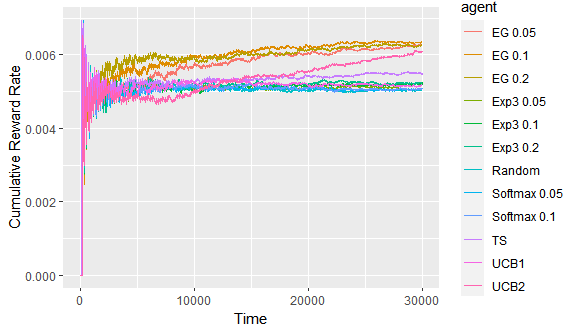
\includegraphics[width=0.49\textwidth]{./figures/SIM-all.png}
    \captionof{figure}{Median cumulative click rate for the bandit algorithms over 100 simulated runs.}\label{fig:SIM-all}
\end{center}

\begin{center}
    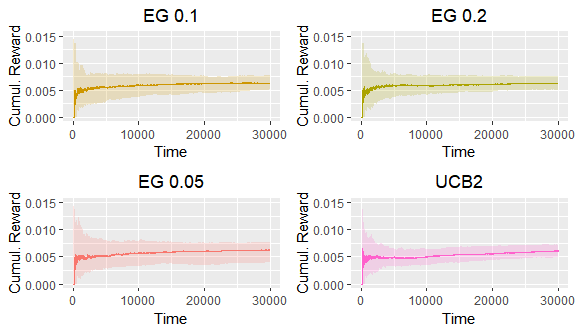
\includegraphics[width=0.49\textwidth]{./figures/SIM-best.png}
    \captionof{figure}{Median cumulative click rate and 95\% pointwise interval for the best four bandit algorithms over 100 simulated runs.}\label{fig:SIM-best}
\end{center}


%##############-####################################################
\color{DarkRed}
\section*{Application to ZOZOTOWN Data}
\color{Black}

\subsection*{Analysis without covariates}

\begin{itemize}
    \item We begin by considering multi-armed bandit policies \textbf{without covariates}.
    
    \item For computational reasons (Algorithm~\ref{alg:Replay Bandit}) the temporal horizon is $T = 12000$.
\end{itemize}



%##############-####################################################

\begin{center}
    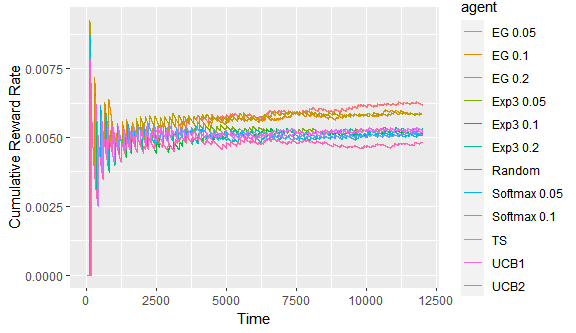
\includegraphics[width=0.49\textwidth]{./figures/RD-all.png}
    \captionof{figure}{Median cumulative click rate for the bandit algorithms over 100 replications of \autoref{alg:Replay Bandit} on random subsets of the data}\label{fig:RD-best}
\end{center}



\end{multicols} 


 %----------------------------------------------------------------------------------------
%	REFERENCES
%----------------------------------------------------------------------------------------
\mbox{}\\[-1.5cm]
\begin{minipage}[c]{0.85\linewidth}
\bibliographystyle{plainnat}
%\bibliography{biblio}
\begin{thebibliography}{}

\bibitem[\protect\citeauthoryear{burtini}{Burtini et~al.}{2020}]{saito2020}
Burtini, G., Loeppky, J. and Lawrence, R. (2015).
\newblock A Survey of Online Experiment Design with the Stochastic Multi-Armed Bandit
\newblock {\em 	arXiv:1510.00757}

\bibitem[\protect\citeauthoryear{saito}{Saito et~al.}{2020}]{saito2020}
Saito, Y., Shunsuke, A., Megumi, M. and Yusuke, N.(2020).
\newblock	Open Bandit Dataset and Pipeline: Towards Realistic and Reproducible Off-Policy Evaluation.
\newblock {\em arXiv:2008.07146.}
\end{thebibliography}
\end{minipage}
\begin{minipage}[c]{0.13\linewidth}
\centering
Scan the QR code below to get to our Git repository!

\includegraphics[scale=0.9]{./figures/frame.png}
\end{minipage}



\end{document}
